\documentclass[oneside, a4paper, twocolumn, reqno, fleqn, 11pt]{article}
\usepackage{style}

\bibliography{biblio}

\usepackage{widetext}

\usepackage[obeyFinal]{todonotes}
% \usepackage{showlabels}

\title{\sc One- and Two-Dimensional Ising Model}
\author{L.E.N. Baakman% 
	\thanks{%
		Master Profile: Computing Science\newline
	 	\hspace*{14pt} Student Number: s1869140%
	}\\%
	\href{mailto:l.e.n.baakman@student.rug.nl}{l.e.n.baakman@student.rug.nl}
}

\begin{document}

\maketitle

\section{Introduction}
\label{s:intro}
%!TEX root = report.tex
A large number of systems change their macroscopic properties at thermal equilibria. For example magnetic atoms align them selves to form a magnetic material at low temperature or high pressure. When modeled mathematically, these phase transitions only occur in infinitely large systems \cite{kenzel1997physics}. This paper investigates a simulation of a finite system, the Ising ferromagnet to be exact.

\Cref{ss:intro:ising} introduces the Ising model of ferromagnetism, the next section discusses the Metropolis Monte Carlo method that is used to estimate the Ising model numerically.

\subsection{Ising Model}
	\label{ss:intro:ising}
	%!TEX root = report.tex
% \todo[inline]{Ising Model in general}
A magnet can be modeled as a large collection of electronic spins. In the Ising model spins point either up, \mbox{\spin{} = +1}, or down, \mbox{\spin{} = -1} \cite{strogatz2014nonlinear}. The magnetization of a magnet is defined as its average spin:
\begin{equation*}
	\magnetization = \abs{\frac{1}{\numberOfSpins} \sum_{i = 1}^{\numberOfSpins} \spin{i}},
\end{equation*}
where \numberOfSpins is the number of spins. At high temperatures the spins point in random directions, consequently the magnetization is approximately zero. At a low enough temperature all spins in the two-dimensional model align themselves, this effect is called spontaneous magnetization. The temperature at which this phase transition occurs is called the critical temperature, \criticalTemperature \cite{cai20011Handout}

\Cref{sss:intro:ising:1D} and \ref{sss:intro:ising:2D} introduce the one- and two-dimensional Ising model, respectively. 

\subsubsection{One-Dimensional Model}
	\label{sss:intro:ising:1D}
	\textcite{ising1925beitrag} introduced a model consisting of a one-dimensional lattice op spin variables. Contrary to the two dimensional model this model does not exhibit state transitions. The Hamiltonian of the one dimensional Ising model with the set spins \mbox{\configuration{} = \spinset} is
	\begin{equation}\label{eq:intro:ising:1D:hamiltonian}
		\hamiltonian\left(\configuration{} \right) = - \interactionStrength \sum_{\pair{i}{j}}\spin{i}\spin{j} - \magneticMoment \sum_{i} \spin{i}.
	\end{equation}
	Where \pair{i}{j} is a nearest neighbour pair, the nearest neighbour of \spin{i} in the one dimensional model are \spin{i - 1} and \spin{i + 1}. \interactionStrength specifies the strength of the interactions between the particles. In a ferromagnetic model, \mbox{$\interactionStrength > 0$} neighboring spins prefer to be parallel. In the anti-ferromagnetic model, \mbox{$\interactionStrength < 0$} spins prefer a direction different to one of their neighbors. The constant \magneticMoment represents the external magnetic field, the spins want to align with the direction of $h$, \ie when \mbox{$h > 0$} spins prefer to be positive. 

	In the following the zero-field ferromagnetic model, \ie \mbox{$\interactionStrength = 1$} and \mbox{$\magneticMoment = 0$},  is considered. The energy \energy of a configuration of spins, \configuration{}, in this model is given by 
	\begin{equation*}
		\energy\left(\configuration{}\right) = \sum_{n = 1}^{\numberOfSpins - 1}\spin{n}\spin{n+1}.
	\end{equation*}
	The probability of a configuration of spins \configuration{} at temperature \temperature is given by
	\begin{equation}
		\label{eq:intro:1D:configurationProbability}
		P\left(\configuration{}\right) = 
		\frac{1}{\partitionfunction} \exp\left[-{E(\configuration{i})}\frac{1}{\temperature}\right],
	\end{equation}
	where $\temperature = \rfrac{1}{\beta}$ and \partitionfunction is the partition function:
	\begin{equation}
		\label{eq:intro:1D:partitionFunction}
		\partitionfunction = \sum_{\spinset} \exp\left[- \energy \beta \right].
	\end{equation}

	% START ANALYTICAL STUFF
	Both the one and two dimensional Ising model can be solved analytically. Under free end boundary conditions, \ie the boundary particles, \spin{1} and \spin{\numberOfSpins}, only observe one neighbor \cite{landau2014guide}, the analytical solution of \cref{eq:intro:1D:partitionFunction} is
	\begin{equation}
		\label{eq:introduced1D:partitionFunctionAnalyticalSolution}
		\partitionfunction = {(2 \cosh \beta)}^\numberOfSpins.
	\end{equation}
	\todo[inline]{Wat is $E_n$?}
	\todo[inline]{Waarover loopt die som?}
	The average energy in the system can be expressed as a function of \partitionfunction \cite{Murray20011Handout}
	\begin{equation*}
		% \label{eq:intro:1D:averageEnergyOriginal}
		\averageEnergy = \frac{1}{\partitionfunction} \cdot \sum_{n} \energy_n \cdot \exp\left[-\beta \energy_n \right].		
	\end{equation*} 
	Observing that
	\begin{equation*}
		\frac{\partial \partitionfunction}{\partial \beta} = \sum_{n} - \energy_n \exp\left[-\beta \energy_n \right],
	\end{equation*}
	and by following the steps presented in \cref{a:derivations:averageEnergy} it can be found that
	\begin{equation*}
		\averageEnergy = - \frac{\partial \ln \left[ \partitionfunction \right]}{\partial \beta} = - \numberOfSpins \cdot \tanh (\beta).
	\end{equation*}
	Consequently $\rfrac{\averageEnergy}{\numberOfSpins} = - \tanh (\beta)$.

	The specific heat describes how the average energy changes as a function of the temperature. Consequently
	\begin{equation*}
		\specificHeat = \frac{\partial \averageEnergy}{\partial \temperature} = \numberOfSpins {\left(\frac{\beta}{\cosh(\beta)}\right)}^{2}
	\end{equation*}
	as shown in \cref{a:derivations:specificHeat} \cite{warkHandout}, consequently
	\begin{equation*}
	 	\frac{\specificHeat}{\numberOfSpins} = {\left(\frac{\beta}{\cosh(\beta)}\right)}^2.
	 \end{equation*}
 
\subsubsection{Two-Dimensional Model}
	\label{sss:intro:ising:2D}
	The 2D Ising model is a square lattice whose lattice sites are occupied by spins. Each spin has either a positive or a negative spin \cite{kenzel1997physics}. The Hamiltonian of the 2D model is the same as the one of the one dimensional model given in \cref{eq:intro:ising:1D:hamiltonian}. The pairs of nearest neighbours are now found by looking at the four connected neighbours, \ie the nearest neighbours of \mbox{spin \spin{i,j}} are \spin{i - 1, j}, \spin{i + 1, j}, \spin{i, j - 1} and \spin{i, j + 1}. \todo{Wat als ie op de rand zit, lopen we rond, of zien we gewoon minder?}The energy of a configuration \configuration{n} that has $\dimensionality \times \dimensionality$ spins is computed as
	\begin{equation}
		\label{eq:intro:ising:2d:energy}
		\begin{split}
		\energy\left(\configuration{n} \right) 
			& = - \sum_{i = 1}^{\dimensionality - 1}\sum_{j = 1}^{\dimensionality} \spin{i,j}\spin{i+1,j}\\
			&\quad\quad - \sum_{i = 1}^{\dimensionality}\sum_{j = 1}^{\dimensionality - 1} \spin{i,j} \spin{i, j+1}.
		\end{split}
	\end{equation}

	% Analytical stuff
	The two-dimensional Ising model has been solved analytically by \textcite{onsager1944crystal}. He showed that the average magnetization per spin on a infinite 2D lattice, \ie $\numberOfSpins = \infty$, is
	\begin{equation}
		\label{eq:intro:ising:2D:magnetizationAnalytical}
		\frac{\magnetization}{\dimensionality^2} = \begin{cases}
			{(1 - {\sinh}^{-4}(2\beta))}^2 & \text{if } \temperature < \criticalTemperature\\
			0 								& \text{if } \temperature > \criticalTemperature
		\end{cases}
	\end{equation}
	where
	\begin{equation*}
		\criticalTemperature = \frac{2}{\ln \left(1 + \sqrt{2}\right)}.
	\end{equation*}

	Given \cref{eq:intro:1D:partitionFunction} solving the the Ising model is relatively simple. To find which configurations of spins result in an equilibirium one only needs to try them all. Unfortunately the computational complexity of this operation is exponential in $\numberOfSpins$, the number of spins. To be exact, a lattice with \numberOfSpins spins has $2^\numberOfSpins$ possible configurations, computing \energy according to \cref{eq:intro:ising:2d:energy} for one configuration takes $2\numberOfSpins$ steps. This leads to $2\numberOfSpins2^\numberOfSpins$ computation steps \cite{kenzel1997physics}. Solving the problem with the Metropolis Monte Carlo method circumvents this complexity problem. 

\subsection{Metropolis Monte Carlo Methods}
	\label{ss:intro:mmc}
	%!TEX root = report.tex

Monte Carlo methods rely on random sampling to obtain numerical results. They are often used to solve problems that might be deterministic in principle but are difficult to solve with other approaches. One of the applications of Monte Carlo experiments is sampling, \ie generating draws from some probability distribution \cite{kroese2014monte}. 

In the context of the Ising model one could naively consider using a few randomly generated states to compute the partition function. However the central limit theorem tells us that these states have an energy that is approximately $\bigOh{\sqrt{\numberOfSpins}}$ for sufficiently large $N$. However the states that we are interested in have an energy of the order \bigOh{\numberOfSpins}, which means that they are not generated at all by the naive method. 

Consequently we need some way to generate the physically relevant states. This can be done by relaxing some configuration into a thermal equilibrium by generating from it a new sequence of states. This requires a transition probability $\transitionProbability\left(\configuration{i} \to \configuration{j} \right)$ from configuration \configuration{i} to configuration \configuration{j}. In thermal equilibrium the probability of finding a given configuration is presented in \cref{eq:intro:1D:configurationProbability}. As we require $P\left(\configuration{i}\right)$ to be stationary in thermal equilibrium we get the detailed balance:
\begin{multline}\label{eq:intro:mcm:detailedbalance}
	\transitionProbability\left(\configuration{i} \to \configuration{j}\right)\exp\left[-\energy(\configuration{i})\beta \right] = \\
	\transitionProbability\left(\configuration{j} \to \configuration{i}\right)\exp\left[-\energy(\configuration{j})\beta \right].
\end{multline}
The function $\transitionProbability(\cdot)$ needs to cover the entire configuration space. The Metropolis algorithm is one of the algorithms that ensures this \cite{kenzel1997physics}. 

This algorithm starts in some initial configuration, it then moves to subsequent configurations by flipping one randomly selected spin with a probability defined by \mbox{$\transitionProbability(\cdot)$}. This is repeated for a given number of steps. Generally one should give the system as number of steps to relax into an interesting state before actually using the generated states.

\todo[inline]{What are we going to discuss in this paper?}

\section{Method}
\label{s:method}
%!TEX root = report.tex
\Cref{alg:method:mmc} presents the pseudo code of the Metropolis Monte Carlo algorithm applied to the Ising problem. This section starts by discussing the input of this algorithm and then introduces the functions used in \cref{alg:method:mmc} one by one. It should be noted that the discussed algorithm is agnostic to the dimensionality of the model. 

%!TEX root = report.tex		
\begin{algorithm}
	\setstretch{1.2}
	\SetAlgoShortEnd
	\DontPrintSemicolon
	\SetKwInOut{Input}{input}\SetKwInOut{Output}{output}
	\Input{
		$\configuration{\mathit{init}}$ the initial configuration\newline
		$\numberOfIterations$ number of iterations
	}
	\BlankLine
	$\configuration{\mathit{cur}}$ := $\configuration{\mathit{init}}$\;
	\For{$i = 0$ \KwTo \numberOfIterations}{
		\spin{} := \FuncSty{selectRandomSpin(\configuration{\mathit{cur}})}\;
		$\configuration{\mathit{pot}}$ := \FuncSty{flipSpin(\spin{}, $\configuration{\mathit{cur}}$)}\;
		$\configuration{\mathit{cur}}$ := \FuncSty{select(
			$\configuration{\mathit{cur}}$,
			$\configuration{\mathit{pot}}$
		)}
	}
	\caption{$\text{MMC}(\configuration{\mathit{init}}, \numberOfIterations)$\label{alg:method:mmc}}
\end{algorithm}

\Cref{alg:method:mmc} requires an initial configuration \configuration{\mathit{init}} as input, this configuration is a representation of the system in its initial state. The parameter \numberOfIterations indicates how many configurations are generated, generally \mbox{\numberOfIterations = \numberOfSpins}. Before the start of the first loop the the current configuration is set to the initial configuration.

$\FuncSty{selectRandomSpin()}$ selects on spin randomly from the spins in \configuration{\mathit{cur}}. The potential configuration, \configuration{\mathit{pot}} is a copy of \configuration{\mathit{cur}} with the selected spin, \spin{}, flipped. This new configuration is generated by \FuncSty{flipSin()}. The new current configuration is selected by \FuncSty{selectConfig()}. The pseudo code of this function is presented in \cref{alg:method:selectConfig}.

%!TEX root = report.tex		
\begin{algorithm}
	\setstretch{1.2}
	\SetAlgoShortEnd
	\DontPrintSemicolon
	\SetKwInOut{Input}{input}
	\SetKwInOut{Output}{output}
	\Input{
			$\configuration{\mathit{cur}}$ the current configuration \newline
			$\configuration{\mathit{pot}}$ the potential configuration
	}
	\Output{
		$\configuration{\mathit{new}}$ the selected configuration
	}

	\BlankLine
	$\Delta \energy$ := \FuncSty{computeDeltaE(
		$\configuration{\mathit{cur}}$, 
		$\configuration{\mathit{pot}}$
	)}\;
	$\xi$ := $\exp\left[- \beta\Delta\energy \right]$\;
	$\theta$ := \FuncSty{randomNumber($0$, $1$)}\;
	\leIf{$\xi > \theta$}{
		$\configuration{\mathit{new}}$ := $\configuration{\mathit{pot}}$\newline
	}{
		$\configuration{\mathit{new}}$ := $\configuration{\mathit{cur}}$
	}
	\caption{$\text{select}(\configuration{\mathit{cur}}, \configuration{\mathit{pot}})$\label{alg:method:selectConfig}}
\end{algorithm}

Given two configurations \FuncSty{selectConfig()} selects with which one the simulation should continue. To this end $\Delta\energy$, the difference in energy between the two configurations, is computed. It is not possible to compute the energy of the two configurations according to \cref{eq:intro:ising:2d:energy}. However writing \cref{eq:intro:ising:1D:hamiltonian} as
	\begin{equation}\label{eq:method:hamiltonian}
			\hamiltonian\left(\configuration{}\right) = - \spin{i} \sum_{j \in \neighbourhood{\spin{i}}} \spin{j} + \mathit{remainder}
	\end{equation}
where $\neighbourhood{\spin{i}}$ is the neighborhood of \spin{i} allows us to see that since only \spin{i} changes the $\mathit{remainder}$ of $\hamiltonian\left(\configuration{\mathit{cur}}\right)$ and $\hamiltonian\left(\configuration{\mathit{pot}}\right)$ are the same \cite{kenzel1997physics}. Thus only the first term in \cref{eq:method:hamiltonian} is relevant for the computation of $\Delta\energy$, consequently we find:
\begin{equation}\label{eq:method:deltaEnergy}
	\Delta\energy = - 2 \cdot \spin{i} \sum_{j \in \neighbourhood{\spin{i}}} \spin{j}.
\end{equation}
If a the potential configuration is determined is decided by two values: $\theta$ and $\xi$. The first is sampled from a pseudo random uniform distribution with the range $\left(0, 1\right)$. The second is computed from $\Delta\energy$ according to
\begin{equation}
	\xi = \exp\left[- \beta\Delta\energy \right].
\end{equation}
If the transition from \configuration{\mathit{cur}} to \configuration{\mathit{pot}} decreases the energy of the system \mbox{$\xi > 1$} and as \mbox{$\theta \in \left(0, 1\right)$} this means that potential states with a lower energy than the current state are always accepted. The guard of the if also ensures that state transitions that increase the energy, \ie \mbox{$\xi < 1$}, are not necessarily discarded.

The implementation of the presented algorithm can be found in \cref{a:implementation}. \todo[inline]{Refer to exact listings.}	

\section{Experiments}
\label{s:experiment}
%!TEX root = report.tex
This section introduces the experiments we ran with the model introduced in the previous sections. In the experiments below the number of iterations, \numberOfIterations, is not necessarily equal to \numberOfSpins, the number of spins, but set independently. To give the system time to relax into the interesting states we perform \mbox{$\rfrac{1}{10} \cdot \numberOfIterations$} Monte Carlo steps, before actually taking the samples used to compute the results. 

 The experiments we ran with the one and two dimensional model are discussed in \cref{ss:experiment:1D,ss:experiment:2D}, respectively.

\subsection{One-Dimensional Model}
\label{ss:experiment:1D}
	In the 1D model we are interested in both the average energy and the specific heat per spin in the following parameter space \mbox{$\temperature = 0.2, 0.4, \dotsc, 4$}, \mbox{$\numberOfSpins=10,100,1000$} and \mbox{$\numberOfIterations=1000,10000$}. 

	\averageEnergy, the average energy is given by
	\begin{equation*}
		\averageEnergy = \frac{1}{\#\sampleSet} \sum_{\configuration{i} \in \sampleSet} E(\configuration{i}),
	\end{equation*}
	where $\sampleSet = \left\{ \configuration{1}, \dotsc, \configuration{\numberOfSamples} \right\}$ is the set of configurations generated during the Monte Carlo steps. \specificHeat, the specific heat is defined as
	\begin{equation*}
		\specificHeat = \beta^2 \left( 
			\frac{1}{\#\sampleSet} \left(  \sum_{\configuration{i} \in \sampleSet} E^2(\configuration{i})\right) - \averageEnergy^2 
		\right).
	\end{equation*}
	Furthermore we will compare the results of the simulation with the analytical solution presented earlier. To compare the numerical and analytical results the mean accuracy of the specific heat and the average energy per spin are computed. The accuracy of a variable where $\nu$ and $\alpha$ represent the numerically and analytically found values, respectively is
	\begin{equation*}
		\accuracy = 1 - \abs{ \frac{\abs{\nu - \alpha}}{\alpha}}.
	\end{equation*}
	\todo[inline]{Refer to listings/section in appendix with the code for this experiment.}

\subsection{Two-Dimensional Model}
\label{ss:experiment:2D}
	In the 2D model we are not only interested in the average energy and specific heat per spin but also the average magnetization per spin. \todo{Formule toevoegen?} The following parameter space is used: \mbox{$\temperature = 0.2, 0.4, \dotsc, 4$}, \mbox{\numberOfSpins = 10, 50, 100} and $\numberOfIterations = 1000, 10000$. The found average average magnetization per spin is compared with the analytical solution presented in \cref{eq:intro:ising:2D:magnetizationAnalytical}.

	\todo[inline]{Refer to listings/section in appendix with the code for this experiment.}	

\section{Results}
\label{s:results}
%!TEX root = report.tex
\todo[inline]{Wat gaan we doen?}

\subsection{One-Dimensional Model}

	\begin{figure*}
		\centering
		\begin{subfigure}{0.49\textwidth}
			\centering
			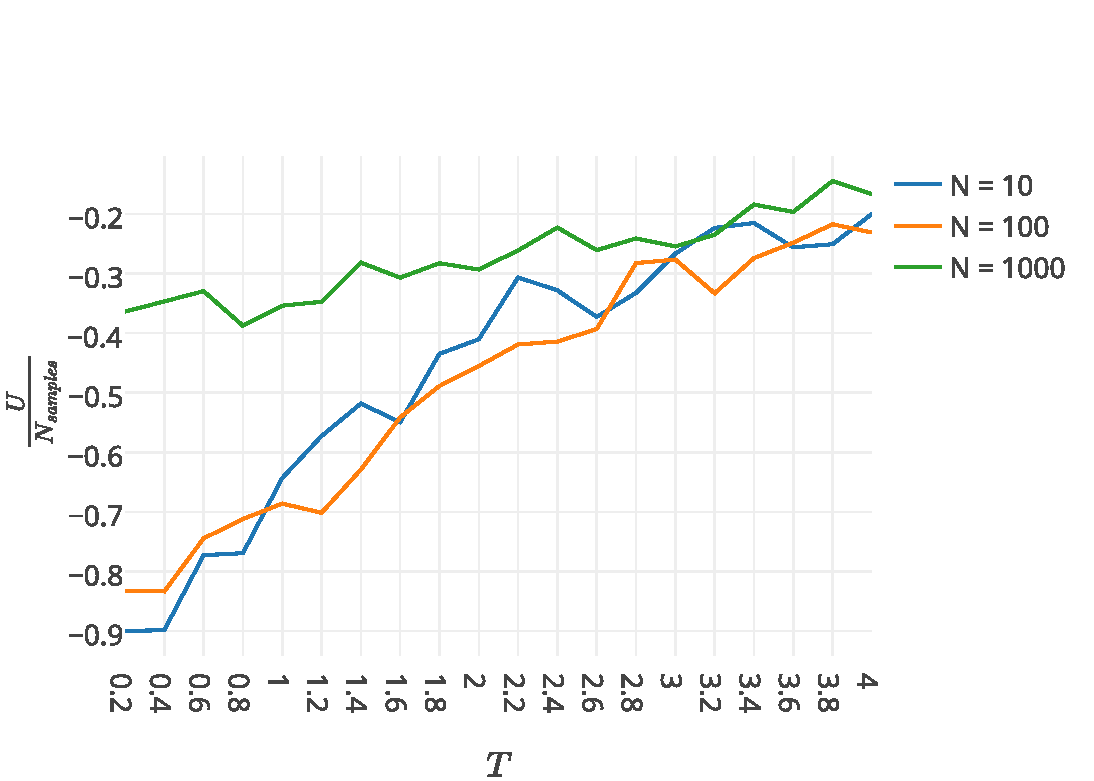
\includegraphics[width=\textwidth, keepaspectratio=true]{img/1D/1DaverageEnergyN1000.pdf}
			\caption{$\numberOfIterations = 1000$}
			\label{fig:results:1D:U:1000}
		\end{subfigure}
		\begin{subfigure}{0.49\textwidth}
			\centering
			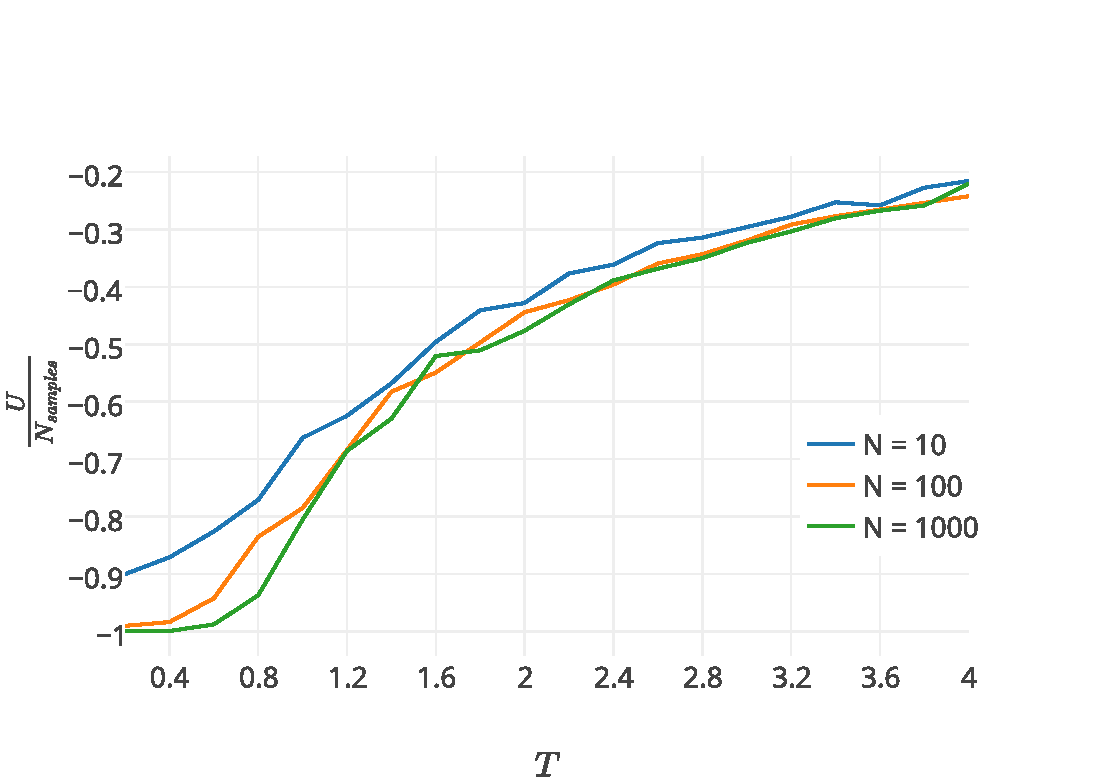
\includegraphics[width=\textwidth, keepaspectratio=true]{img/1D/1DaverageEnergyN10000.pdf}
			\caption{$\numberOfIterations = 10000$}
			\label{fig:results:1D:U:10000}
		\end{subfigure}	
		\caption{The average energy for \subref{fig:results:1D:U:1000} 1000 and \subref{fig:results:1D:U:10000} 10000 sample iterations.}
		\label{fig:results:1D:U}
	\end{figure*}

	\subsubsection{Average Energy}
		\todo[inline]{Report average energy for different values of T, N and NSAMPLES}

	\subsection{Specific Heat}
		\todo[inline]{Report specific heat for different values of T, N and NSAMPLES}

\subsection{Two-Dimensional Model}
	\todo[inline]{Wat gaan we doen?}

	\subsubsection*{Average Energy}
		\todo[inline]{Report average energy for different values of T, N and NSAMPLES}


	\subsubsection*{Specific Heat}
		\todo[inline]{Report specific heat for different values of T, N and NSAMPLES}

	\subsubsection*{Average Magnetization}
		\todo[inline]{Report average magnetization for different values of T, N and NSAMPLES}	

\section{Discussion}
\label{s:discussion}
%!TEX root = report.tex
In this section the results of the two experiments, presented in \cref{s:results}, are discussed.

\subsection{One-Dimensional Model}
	
	We have observed that the accuracy increases as the temperature increases and that at very low temperatures the accuracy is very low. This is caused by the Boltzman factor, which is low when the \temperature is low. Thus very few potential states are accepted at a low temperature. Consequently the system `moves slower' and takes longer to end up in the interesting states.
	
	The results in \cref{a:results1D} showed that the accuracy increases as the number of samples increases. The cause for this is that the analytical solutions are based on systems with an infinite number of spins. Consequently system with more spins are closer to systems with $\numberOfSpins = \infty$, and their results are thus closer to those of the infinite system. 

	Another factor that increases the accuracy of the system is the number of samples. Firstly more samples means that the system gets more time to relax. Secondly a higher number of samples decreases the influence of outlier states. Lastly the probability of ending up in a interesting configuration increases as the number of spins that are potentially flipped increases.

	As expected we do not observe a phase transition in the one-dimensional model. 

\subsection{Two-Dimensional Model}
	In line with the theory we have observed that there is a phase transition and that it is approximately critical. In the systems with few spins, $\dimensionality = 10$, the phase transition is hardly visible in the plots. This is due to the analytical results being based on infinite systems. 

	Unfortunately we cannot offer an explanation for the drop in magnetization at $\temperature = 2.1$ in the $10 \times 10$ system with 1000 samples.

\section{Conclusion}
\label{s:conclusion}
%!TEX root = report.tex
Our findings have shown that even a small two-dimensional system with a relatively small number of samples is sufficient to observe a phase transition. However to get results that approximate the analytical solutions of the Ising model one needs to make sure that the system is suffieciently large. Furthermore one should allow the system a reasonable number of Monte Carlo steps to relax and take a large number of samples. 


\printbibliography

\onecolumn
\allowdisplaybreaks %Allow the breaking of math environments.

\appendix
\section{Mathematical Derivations}
\label{a:derivations}
%!TEX root = report.tex
\subsection{Average Energy}
	\label{a:derivations:averageEnergy}
	\begin{align*}
		\averageEnergy 
			& = - \frac{\partial \ln \left[ \partitionfunction \right]}{\partial \beta}.\\
		\comment{
			\textit{Definition of \partitionfunction in \cref{eq:introduced1D:partitionFunctionAnalyticalSolution}}.
		}
		\content{
			- \frac{\partial \ln \left[ \left(2 \cosh \beta \right)^N \right]}{\partial \beta}
		}
		\comment{
			\textit{Chain rule: } 
			\frac{\partial}{\partial \beta}\ln\left[2^N \cosh^N(\beta) \right] = \frac{\partial \ln\left[ u \right]}{\partial u} 0, \, 
			u = 2^n \cosh^n(\beta),\,
			\frac{\partial}{\partial u} \ln\left[ u \right] = \frac{1}{u}
		}
		\content{
			- 2^{-N} \cosh^{-N}(\beta) \left( \frac{\partial}{\partial \beta} \left( 2^N \cosh^N(\beta)\right)\right)
		}
		\comment{
			\textit{Factor out constants.}
		}
		\content{
 			- 2^{- N} \frac{\partial}{\partial \beta}\left(\cosh^{N}(\beta)\right) 2^{N} \cosh^{-N}(\beta)
		}
		\comment{
			\textit{Simplify the expression.}
		}
		\content{
			-\cosh(\beta) ^{-N} \left(\frac{\partial}{\partial \beta} \cosh^{N}(\beta)\right)
		}
		\comment{
			\textit{Chain rule: } \frac{\partial}{\partial \beta} \cosh^{N}(\beta)=\frac{\partial u^N}{\partial u} 0,\, 
			u = \cosh(\beta),\, 
			\frac{\partial}{\partial u}\left(u^N\right) = N \cdot u^{-1 + N}
		}
		\content{
			- N \cosh(\beta)^{N-1} \frac{\partial}{\partial \beta}\left( \cosh (\beta) \right) \cosh^{-N} (\beta)
		}
		\comment{
			\textit{Simplify the expression.}
		}
		\content{
			- N \left(\frac{\partial}{\partial \beta} \cosh(\beta) \right) \text{sech}(\beta)
		}
		\comment{
			\textit{Derivative of } \cosh(\alpha) \textit{ is } \sinh(\alpha).
		}
		\content{
			- \sinh(\beta) N \text{sech}(\beta)
		}
		\comment{
			\textit{Simplify the expression.}
		}
		\content{
		- N \tanh(\beta)
		}
	\end{align*}

% \subsection{Specific Heat}
% 	\label{a:derivations:specificHeat}
% 	\begin{align*}
% 		\specificHeat 
% 			& = \\
% 		\comment{
% 			\textit{Some comment}.
% 		}
% 		\content{
% 			b
% 		}
% 	\end{align*}

\section{Implementation}
\label{a:implementation}
%!TEX root = report.tex

\subsection{Simulation}
\label{app:implementation:simulation}
	\lstinputlisting[label={lst:simulation:mmci}]{./../code/MMCIsing.m}
	\lstinputlisting[label={lst:simulation:neighbours1d}]{./../code/+neighbors/OneD2Connected.m}
	\lstinputlisting[label={lst:simulation:neighbours2d}]{./../code/+neighbors/TwoD4Connected.m}

\subsection{Statistics}
\label{app:implementation:statistics}
	\lstinputlisting[label={lst:statistics:computeAverageEnergy}]{./../code/computeAverageEnergy.m}
	\lstinputlisting[label={lst:statistics:computeSpecificHeat}]{./../code/computeSpecificHeat.m}
	\lstinputlisting[label={lst:statistics:computeAccuracy}]{./../code/computeAccuracy.m}
	\lstinputlisting[label={lst:statistics:computeMagnetization}]{./../code/computeAverageMagnetization.m}


\subsection{Experiments}
\label{app:implementation:experiments}
	\lstinputlisting[label={lst:experiment:1d}]{./../code/experiment_1D.m}
	\lstinputlisting[label={lst:experiment:2d}]{./../code/experiment_2D.m}

\subsection{Plots}
\label{app:implementation:plots}
	\lstinputlisting{./../code/plot_1D.m}
	\lstinputlisting{./../code/plot_2D.m}
	\lstinputlisting{./../code/+output/averageEnergy1D.m}
	\lstinputlisting{./../code/+output/specificHeat1D.m}
	\lstinputlisting{./../code/+output/private/filterExperiments.m}

\subsection{Tables}
\label{app:implementation:tables}
	\lstinputlisting{./../code/tables_1D.m}
	\lstinputlisting{./../code/tables_2D.m}
	\lstinputlisting{./../code/+output/generateLaTeXTable.m}
	\lstinputlisting{./../code/+output/collectData.m}


\end{document}